\chapter{Specification}
The specification of the program defines what it does rather than how.
This chapter presents the specification of the system taking into consideration general software engineering principles, like the models proposed by Larman (FIXME CITE??)(at least conceptual, use case and behaviour models) and Meyer's (FIXME CITE??) \ac{DbC}.
For the particular case of this thesis, the specification takes into account reengineering principles and procedures and \ac{TDD} as a tool to define what the system does as opposed to a simple testing technique.

Reengeneering software comprises 6 activities (TODO Maybe cross ref chapter 2): 
\begin{enumerate}
    \item Inventory Analysis
    \item Documentation reestructure (FIXME Language)
    \item Reverse Engineering
    \item Code Restructuring
    \item Data Restructuring
    \item Forward Engineering
\end{enumerate}   
   
The outcome of these activities (FIXME: activity, task?) derives part of this specification.
For example, use cases are extracted from the current system.
The first three focus on what the system does and are used in this chapter, whereas the last three are tightly coupled to technology and are expanded in chapter design (FIXME cross ref chapter 6?).

\section{Inventory Analysis}
A sorted list of software in the organisation makes candidates for reengeneering appear.
The scope of this thesis is reengineering Flango in the robot and it is a decision taken before starting this work.
However, Flango uses other software that might have to be reengineered in the future or even modified to suit the needs of the new technology in the project.

\begin{inventory}
{name=Flango Frontend (robot), 
year=May 2011,
nchanges=5 big milestones,
lastchange=August 2013,
sysresides=Reem H2 and H3,
appinterfaces=Flango Backend; robotBehaviour,
dbs=SQLite in the robot (exclusive use),
errors=not tracked,
nusers=all employees (+40) and business leads (at least one per week),
ninstallations=3 (one per dev robot in the office),
complexityArch=Simple (MVC),
complexityCode=Medium (custom \ac{XML} parser),
complexityDocs=No documentation,
qualityDocs=N/A,
overallMainten=One software engineer full-time (extension and maintenance),
projLongevity=Until September 2013,
projNchanges36=0,
maintenCost=1 software engineer full-time,
operCost=no exclusive cost,
bizVal=high (no revenue generated yet but it can be sold without the robot),
bizCrit=very high (contents have big impact: they belong to the \ac{UI})
}
\end{inventory}

\begin{inventory}
{
name=Flango Screens Editor, 
year=December 2012,
nchanges=4 (first version; some new features; bug fixing),
lastchange=August 2013,
sysresides=Basestation,
appinterfaces=Flango Frontend (robot); Flango Backend,
dbs=flango (postgresql through the Backend),
errors=not tracked,
nusers=business department (+5 people) and a some software engineers (+7),
ninstallations=2,
complexityArch=Simple (MVC),
complexityCode=Medium (large ActionScript codebase and custom \ac{XML} parser),
complexityDocs=No documentation,
qualityDocs=N/A,
overallMainten=1 software engineer full-time,
projLongevity=At least until January 2015,
projNchanges36=Bug fixing,
maintenCost=1 software engineer full-time,
operCost=no exclusive cost,
bizVal=high (no revenue generated yet but it can be sold without the robot),
bizCrit=very high (contents have big impact: they belong to the \ac{UI})
}
\end{inventory}

\begin{inventory}
{
name=Flango Backend, 
year=October 2012,
nchanges=3 (first version; statistics; new features),
lastchange=August 2013,
sysresides=Basestation,
appinterfaces=Flango Frontend (robot); Flango Screens Editor,
dbs=flango (postgresql),
errors=not tracked,
nusers=business department (+5 people) and a some software engineers (+7),
ninstallations=2,
complexityArch=Simple ("MVC"),
complexityCode=Medium (large Django codebase),
complexityDocs=Simple for this project,
qualityDocs=Very high for Django; Poor for Flango Backend,
overallMainten=1 software engineer full-time,
projLongevity=At least until January 2015,
projNchanges36=Unspecified number of new features and bug fixing,
maintenCost=1 software engineer full-time,
operCost=no exclusive cost,
bizVal=high (no revenue generated yet but it can be sold without the robot),
bizCrit=very high (contents have big impact: they belong to the \ac{UI})
}
\end{inventory}    

    
    The following checklist may help to determine which applications are candidates for reengineering. The more questions that receive a positive ("yes") response, the higher the probability that the application is a candidate for reengineering.

    Is the application more than five years old?
    Is the application business critical?
    Is the project longevity projected to be more than five years?
    Is the number of users large by local standards?
    Is the number of users likely to increase?
    Are major changes contemplated for the application?
    If so, will these major changes require substantial commitent of effort by local standards?
    Is the cost of continuing annual maintenance known?
    Is the annual value of the application known?
    Is the projected total cost of change known?
    Can the cost to reengineer the application be estimated to within 20%?
    If so, is reengineering cost less than the cost to make changes plus the cost of maintenance?

\section{Document Reestructure}
maybe we don't need this.

\section{Reverse Engineering}
\label{sec:context}
Reengineering a software involves reverse engineering, understanding what the system does.

There are 3 key issues in understanding the current system: abstraction level, completeness and direction.
This specification uses a system-level abstraction, only takes into account interaction with external actors, and is one-way (from current system to the specification of the new system).
Other levels of abstraction do not apply here to keep this specification technology-agnostic.

\subsection{Context}
\begin{figure}[htb]
    \centering
    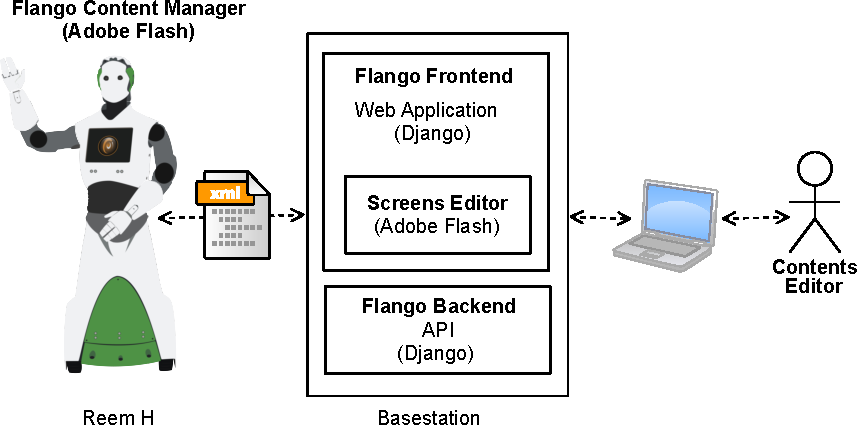
\includegraphics[width=\textwidth]{figures/context-original}
    \caption{Current context}
    \label{fig:context-original}
\end{figure}

\begin{figure}[htb]
    \centering
    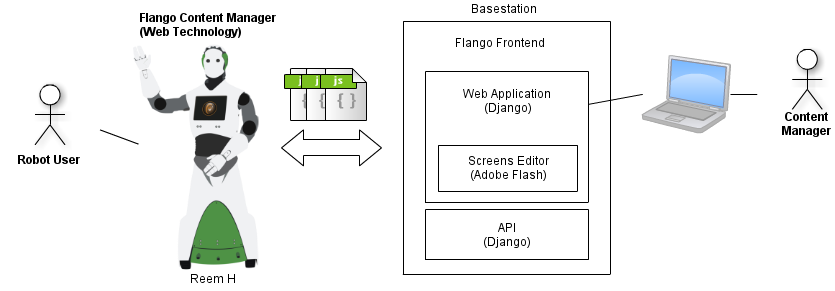
\includegraphics[width=\textwidth]{figures/context-new}
    \caption{New context}
    \label{fig:context-new}
\end{figure}

ReemH-3 has about 600MB of specialised code and uses up to 13GB to store the operating system, libraries and other tools.
The program that manages the state machine is \textbf{robotBehaviour}, a \texttt{Qt} program that glues all software parts and serves as an interface to the hardware.
A window in this program contains a QtWebKit widget (FIXME maybe chrome!), the embedded web browser that loads the contents in the touchscreen.
Contents are fetched from Basestation, a server that hosts \textbf{Flango Frontend}, a web application (Django + Flash) that lets users edit screens, add media contents and synchronise them with robots (\fref{fig:context-original}).
The Frontend has an \ac{API} to serve the contents applications to the robots.
The project of this thesis is reengineering the \textbf{Flango Content Manager}, in the robot (\fref{fig:context-new}).

\subsection{Interaction}
\begin{figure}[htb]
    \centering
    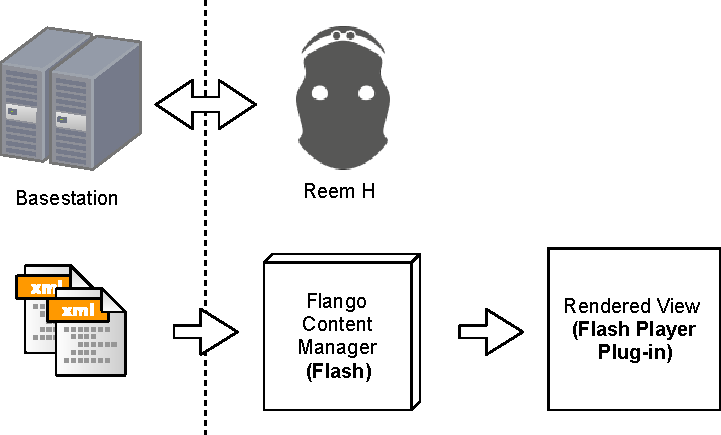
\includegraphics[width=0.7\textwidth]{figures/interaction-original}
    \caption{Current interaction}
    \label{fig:interaction-original}
\end{figure}

\begin{figure}[htb]
    \centering
    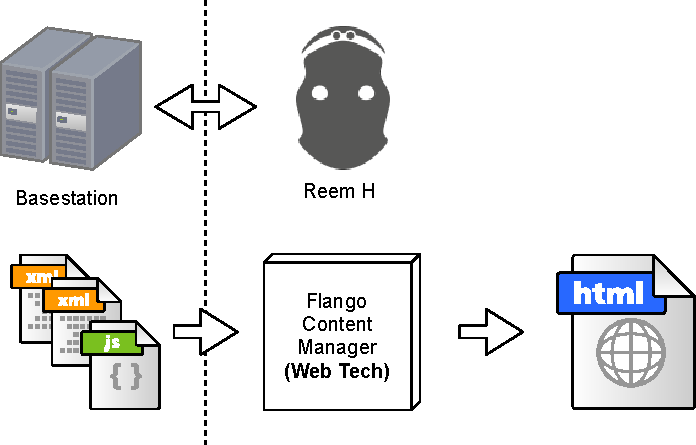
\includegraphics[width=0.7\textwidth]{figures/interaction-new}
    \caption{New interaction}
    \label{fig:interaction-new}
\end{figure}

The content manager's input is \ac{XML} code and the output is an \ac{HTML} single page application (\fref{fig:interaction-original} and \fref{fig:interaction-new}).
The general boot steps are:

\begin{enumerate}
    \item The robot boots
    \item robotBehaviour fetches settings (\ac{XML}) from Basestation: generic settings, contents application-specific settings and the structure.
    \item The Content Manager uses the settings to decide which application to load, the language, the theme, etc. and requests the screens (the \ac{XML} files) to Basestation
    \item Basestation serves all the screens
    \item The Content Manager renders the screens. If during this process encounters an "entity", it fetches the data from Basestation.
\end{enumerate}


\subsection{Interoperability}
\begin{figure}[htb]
    \centering
    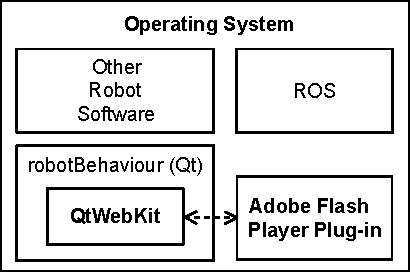
\includegraphics[width=0.7\textwidth]{figures/interoperability-original}
    \caption{Current interoperability (in robot)}
    \label{fig:interoperability-original}
\end{figure}

\begin{figure}[htb]
    \centering
    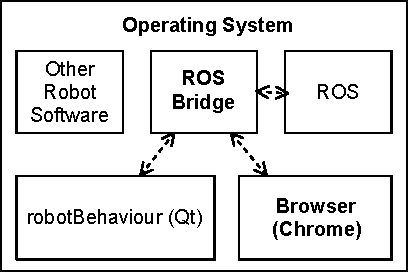
\includegraphics[width=0.7\textwidth]{figures/interoperability-new}
    \caption{New interoperability (in robot)}
    \label{fig:interoperability-new}
\end{figure}

Flango Content Manager interoperates with two systems: robotBehaviour and Basestation.

\paragraph{robotBehaviour} Flango can interact with the hardware of the robot through robotBehaviour, e.g. using text-to-speech capabilities, triggering a batch action (autopresentation, guide user to a certain place...).
Likewise, robotBehaviour uses an API in Flango, e.g. to restart a session or to input information gathered with the robot's hardware.
There is an interface defined for this to allow independent development in both ends.
Notice that figures \fref{fig:interoperability-original} and \fref{fig:interoperability-new} do not show Basestation. See \fref{fig:context-original} and \fref{fig:context-new}.
The current system to exchange messages between the Flash container and robotBehaviour is based on JavaScript callbacks.
To send a message to robotBehaviour:
\begin{enumerate}
    \item Flash opens a new tab with a specific url: \texttt{flashCallback.html?\textless paramList\textgreater}
    \item robotBehaviour intercepts the call, prevents QtWebKit from opening a new tab and executes an action specified with the parameters
\end{enumerate}

To send a message from robotBehaviour:
\begin{enumerate}
    \item Calls a \ac{JS} function in the Flash container (\texttt{/static/frontend/index.html})
    \item The container forwards this call to the Flash container
    \item The application facade of Flango Content Manager takes required action
\end{enumerate}

The requirements state that the new software has to be implemented using web technology. 
Despite the fact that this specification should be technology agnostic, to integrate the new software better in the system, the use of ROS Web Tools is suggested to exchange messages.
In any case, it is clear that there has to be an interface between robotBehaviour and the browser, as they run in separate processes (as opposed to sharing at least one parent process in the current implementation).

\paragraph{BaseStation (Flango Backend API} The Content Manager has to fetch data from Basestation in order to load the correct contents.
Flango Backend (TODO EPIC FIXME. fix the diagrams and everything. BS has backend and frontend) has an API for this (\fref{tab:flango-api}):

\begin{table}[ht]
    \centering
    \begin{tabularx}{\linewidth}{| l | X |}
    \hline
    Root URL & Matching URLs \\
    \hline
    \multirow{2}{*}{\texttt{flango-api-0.1/robots}}
        & get\_robots \\ 
        & add\_robot \\
    \hline 
    
    \multirow{2}{*}{\texttt{flango-api-0.1/bl}} 
        & entity/(\textless entity\_name\textgreater).xml \\ 
        & add\_robot \\
    \hline
    
    \multirow{6}{*}{\texttt{flango-api-0.1/pal}} 
        & home \\
        & add \\
        & execute \\
        & status \\   
        & submit \\
        & history/(\textless page\textgreater) \\
    \hline
    
    \multirow{10}{2.5cm}{\texttt{flango-api-0.1/gui}  \texttt{flango-api-0.1/app}}
        & \textless app\_id\textgreater /config.\textless format\textgreater xml$|$json \\
        & \textless app\_id\textgreater /structure.\textless format\textgreater xml$|$json \\
        & \textless app\_id\textgreater /screen/( \textless screen\_id\textgreater.xml \\
        & \textless app\_id\textgreater /node/\textless node\_id\textgreater \\
        & application \\
        & node \\
        & screen \\
        & allScreens \\
        & getApps \\
        & upload\_app \\
    \hline
    
    \multirow{7}{*}{\texttt{flango-api-0.1/stats}}
        & robot/use/<robotID>/<duration>/<data> \\
        & robot/base \\
        & app/use/<robotID>/<duration>/<data> \\
        & app/top/<robotID>/<duration>/<data> \\
        & app/toptable/<page> \\
        & application/<screen> \\
        & <name> \\
    \hline
    \end{tabularx}
    \caption{Flango Backend API}
    \label{tab:flango-api}
\end{table}
Both current and new implementation use this.
However, the new implementation uses \ac{JSON} because it is more \ac{JS}-friendly: it has less overhead and it is easier to deserialise.


\section{Conceptual Model}
TODO FIXME subindex in captions
\begin{sidewaysfigure}[htb]   
    \centering
    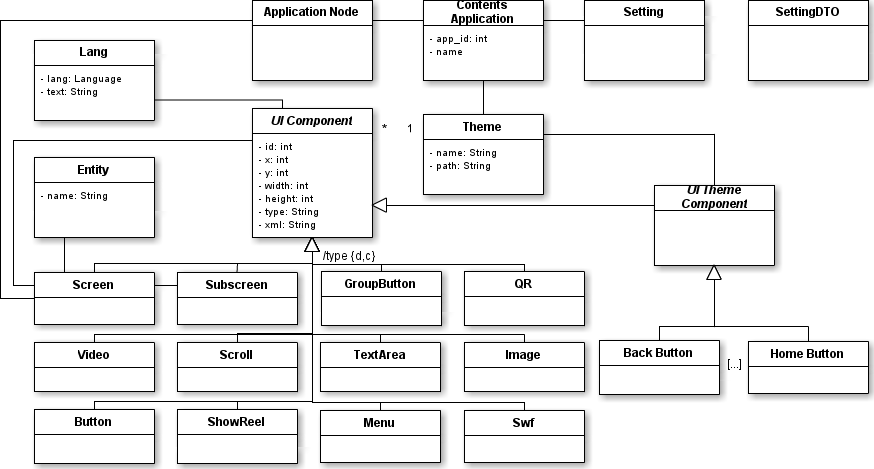
\includegraphics[width=\textwidth]{figures/specification-conceptual-model}
    \caption{Conceptual model}
    \label{fig:specification-conceptual-model}
\end{sidewaysfigure}

There are only a few classes of objects in the system.
This project only reengineers Flango Content Manager.
Because the Screens Editor (Flango Frontend) remains "as is", and the input of the new software is the output of this program, it has to be compatible with the current implementation.
Otherwise, users would create contents applications with the Screens Editor that would look different when they are displayed in the robot.
To ensure compatibility, it is necessary a good understanding not only at system level, but at component level.
It is required, then, that the new implementation can render consistently all of the \ac{UI} components that the Screens Editor can create and all of their properties. 
Same applies to settings and use of "entities".
Thus, there are at least 3 classes of objects: Setting, UI Component (and UI Theme Component), Entity.

A UI Component is an element of the \ac{UI}, for example a Button or an Image.
Users drag and drop them to a canvas in the Screens Editor to create the contents. 
All UI Components have an \ac{XML} code.
Because the domain of the problem and the classes are shared between the original and the new implementation, the model in \fref{fig:specification-conceptual-model} is created from the current implementation.
To support themes, there are two types of UI Components: basic (UI Component) and theme (UI Theme Component).
All UI Theme Component are eventually implemented with a basic UI Component.

\begin{lstlisting}[caption=Basic UI Components, label=onelabel]
ButtonComponent.as
GroupButtonComponent.as
GroupComponent.as
ImageComponent.as
MenuComponent.as
QRComponent.as
ScreenComponent.as
ScrollComponent.as
ShowReelComponent.as
SubscreenComponent.as
SWFComponent.as
TextareaComponent.as
UIComponent.as
VideoComponent.as
\end{lstlisting}

\begin{lstlisting}[caption=Theme UI Components, label=anotherlabel]
arabic_button
back_button
base_button
big_button
call_to_action_screen
camera_button
config_button
english_button
forward_button
home_button
info_button
korean_button
language_button
left_arrow_button
line
list_button
main_menu
next_button
reem_body_button
reem_button
right_arrow_button
smartphone_menu
synchronizing_screen
video_button
wide_button
\end{lstlisting}

\begin{lstlisting}[caption=Application State (Settings class), label=anotherlabel2]
api_endpoint:String
app_id:String
app_name:String
current_node:String
debug_level:String
debug_mode:Boolean
default_api_endpoint:String
def_lang:String
def_theme:String
enable_stats_bkp:Boolean
enable_stats:Boolean
history:Array
history_current:int
history_limit:int
home_node:String
initial_node:String
lang_list:Object
lang:String
log:String
media_path:String
performance_monitor:Boolean
perform_callbacks_bkp:Boolean
perform_callbacks:Boolean
redirects:Array
report_stats:Boolean
robot_id:String
scale_factor:Number
screensaver_node:String
screens:Object
screen_transitions:Boolean
security_level:int
session_fadeout:int
session_timeout:int
show_cursor:Boolean
static_api_endpoint:String
static_media_path:String
static_themes_path:String
structure:XML
theme_list:Object
themes_path:String
theme:String
themes:XMLList
zone:String

\end{lstlisting}

\ref{onelabel} and \ref{anotherlabel} contain a comprehensive list of UI Components extracted from listing the necessary files in a package of the current implementation.
Notice that all files in \ref{onelabel} have the corresponding class in the conceptual model.
The elements of \ref{anotherlabel} are in fact folders but they can be considered objects in this specification as they are part of the domain of the problem.
The state of the application is defined with DTOs sent from the server.
A collection of the necessary the attributes of the class that encapsulates the configuration is in \ref{anotherlabel1} and has been extracted from the current implementation as well.

Entities are classes that represent classes in the Screens Editor. 
Imagine the following scenario: Alice is creating screens with the Screens Editor.
She rented the robot for a congress and wants to add information about job openings in her company.
She can define, with Flango, an entity named "Job" and use it in the screens editor to show the list of all instances of Job.

A Contents Application can have themes.
There is a default theme that defines the look and feel of all UI Theme Components.
All themes have the same UI Theme Components to guarantee that themes can be changed safely.
Basic UI Components look always the same way.

TODO explain XML here? explain theming here? fallbacks? ambiguity?

TODO : maybe --- I can't remember what I was going to write here.
For instance, the \ac{XML} code of a Button UI Component in \fref{chap:specification-button-example-1}

\lstinputlisting[language=XML, caption={Basic UI Component Button XML}]{src/specification-button-example-1.xml}

DIAGRAM HERE


constraints?

\section{Use Case Model}
This section describes the services of the system as sequences of events triggered by external actors.

\subsection{Actors}
Humans only interact directly with the output of this software (see \fref{sec:context}), which becomes the \ac{GUI}.
For example: the program renders a screen with one button whose action is to make Reem say "hi, my name is Reem".
The input is an \ac{XML} file, the output is a web \ac{GUI} ready to be used.
Humans can now touch the button that sends events to robotBehaviour so, essentially, the \ac{GUI} of the program and not only the output is built as a function of the input.
The actual actors are robotBehaviour, the Flango Backend  and, eventually, a user of the contents.


\subsection{System Use Cases}

\begin{figure}[htb]  
    \centering
    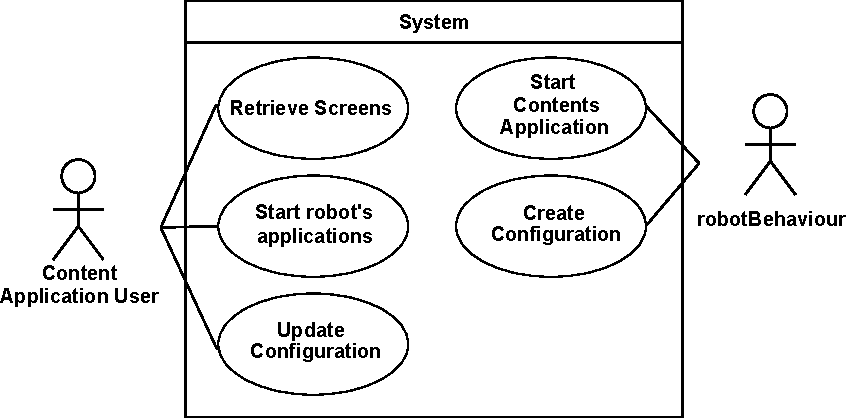
\includegraphics[width=\linewidth]{figures/specification-sucs}
    \caption{System Use Cases}
    \label{fig:specification-sucs}
\end{figure}

There is a number of use cases of the software determined by examining the current implementation at a program level.
The use cases that are implemented in this project are shown in \fref{fig:specification-sucs}.

A contents application user can see the rendered screens and manipulate it (e.g. change the language).
For an application to load the configuration has to be fetched from Flango Backend.
A user can also start other applications in the robot.
For example: the user touches a button that makes Reem say a sentence aloud (notice that the application is sending a message to robotBehaviour).
The software system that controls the robot, robotBehaviour, can also trigger actions in the contents application.
Amongst others, it can manage the screensaver and sessions and some special settings (including: show the cursor, enable debug mode, enable sending message to robotBehaviour, contents application ID, etc)




\section{Behaviour Model}
seq diagrams of system operations

This thesis combines \ac{DbC} and \ac{TDD}, two techniques that are not mutually exclusive.
Basically, tests define the behaviour for specific cases and \ac{DbC} defines the general behaviour. 
Thus, there are no tests for edge cases or negative behaviours because contracts, and more specifically preconditions, protect the component.
In spite of the name, \ac{TDD} tests are executable specifications.
They become tests only after having implemented all the functionality being test-driven.
Before this, there is nothing to actually test and these artifacts are rather executable specifications, but not tests.
Tests (specifications) are written before the code and define the behaviour of components.

Additionally, they are used as documentation of the program but they are not sufficient to completely define the behaviour because they only assert properties by example instead of stating general properties (e.g. "it should return 5" vs "return value $1 \leq x \leq 10$"). The latter can be achieved using formal specifications,
e.g. using Meyer's \ac{DbC} \cite{Baumeister:2004}.

In this thesis, tests are implemented with Jasmine and AngularJS but this chapter focuses on what the tests describe rather than how they are executed and controlled.

Combining the two techniques one can use the best parts of each to define the behaviour of the system.
With \ac{TDD}:
\begin{itemize}
    \item Build only what is required (Keep it simple and control the scope of the project)
    \item Drive design decisions from tests (i.e. from the specification)
\end{itemize}

With formal specifications (\ac{DbC}):
\begin{itemize}
    \item Higher code quality
    \item Less checks (preconditions)
    \item Drive design decisions from preconditions
\end{itemize}


Larman: system sequence diagram + Meyer: contracts of system operations
"System Sequence Diagrams:
–
Identify system events and system operations
–
Identify system events and system operations
– Document sequence of interactions
• Contracts:
– Define the pre- and post-conditions for system
operations "

up to date documentation: a common problem is that docs are hardly ever updated

\section{XML Representation}
explain syntax here?